\documentclass[conference]{IEEEtran}
\IEEEoverridecommandlockouts
% The preceding line is only needed to identify funding in the first footnote. If that is unneeded, please comment it out.
%Template version as of 6/27/2024

\usepackage{cite}
\usepackage{amsmath,amssymb,amsfonts}
\usepackage{algorithm}
\usepackage{algorithmic}
\usepackage{graphicx}
\usepackage{textcomp}
\usepackage{xcolor}
\usepackage{float}
% \usepackage[hidelinks]{hyperref}
\definecolor{softblue}{RGB}{100,149,237}
\usepackage[colorlinks=true, linkcolor=black, citecolor=black, urlcolor=softblue]{hyperref}
\def\BibTeX{{\rm B\kern-.05em{\sc i\kern-.025em b}\kern-.08em
    T\kern-.1667em\lower.7ex\hbox{E}\kern-.125emX}}
\begin{document}

% ________________________________________________________________________________________________________________

% TITLE
\title{Efficient Transformer Compression in Pre-trained Language Models Through Selective Tensor Rank Reduction\\
}

\author{\IEEEauthorblockN{Made Branenda Jordhy}
\IEEEauthorblockA{ Informatics Engineering Study Program \\
School of Electrical Engineering and Informatics\\
Bandung Institute of Technology, 10 Ganesha Street, Bandung\\
E-mail: \href{mailto:ethgalleryin@gmail.com}{ethgalleryin@gmail.com}, \href{mailto:13524026@std.stei.itb.ac.id}{13524026@std.stei.itb.ac.id}}
}

\maketitle

% ________________________________________________________________________________________________________________

% ABSTRACT
\begin{abstract}
Large language models (LLMs) and transformer based architectures have become prevalent in natural language processing, 
yet their massive parameter count limits deployment in resource constrained environments. This paper investigates 
tensor rank reduction as a structured compression technique to address inference latency and memory consumption 
while preserving model performance. We apply selective tensor decomposition, specifically Tucker and Tensor-Train 
factorization, to compress weight matrices in transformer feed forward networks and attention layers of pre-trained 
language models. Our approach balances computational efficiency with model expressiveness through careful per-layer 
rank selection. Experiments on a small scale transformer for sentiment analysis demonstrate that selective tensor 
decomposition achieves 30–50\% parameter reduction in targeted layers with less than 2\% accuracy loss and 
approximately 25–35\% inference speedup. Analysis reveals that different layer types respond differently to 
decomposition and that low-rank approximations effectively preserve linguistic information. Our findings suggest 
tensor-based compression is a practical complementary approach to quantization and pruning for deploying 
language models on edge devices.
\end{abstract}

\begin{IEEEkeywords}
tensor decomposition, model compression, transformer efficiency, natural language processing, low-rank approximation
\end{IEEEkeywords}

% ________________________________________________________________________________________________________________

% INTRODUCTION
\section{Introduction}

% Background
\subsection{Background}
Large language models (LLMs) such as ChatGPT and BERT have achieved remarkable performance on natural language processing tasks.
However, their massive parameter counts, often billions, require substantial computational resources, making deployment in
resource-constrained environments difficult. For example, models like GPT-3 demand high-end GPUs or TPUs and result in significant
infrastructure costs. Inference latency and memory consumtion also create bottlenecks for real time applications like chatbots
and recommendation systems. 

To reduce these computational demands, several compression techniques have been proposed, like quantization reduces numerical
precision, pruning removes less important parameter, and knowledge distillation trains smaller models to imitate larger ones.
Each approach has limitations. Quantization introduces numerical errors, pruning creates irregular sparse patterns that are hard to
accelarate, and distillation requires additional training. Tensor decomposition offers and alternative approach by approximating
weight matrices as low rank tensor products, reducing parameters while maintaining structured, hardware friendly patterns. Unlike
pruning and quantization, tensor based methods exploit the inherent low rank structure of transformer weights through mathematical
factorization and offering complementary compression strategy.

% Research Objectives
\subsection{Research Objectives}
This paper investigates tensor rank reduction, specifically Tucker and Tensor-Train decomposition, to compress transformer based
language models. Our main contributors are a systematic analysis of how tensor decomposition methods apply to transformer feed 
forward and attention layer, selective layer wise decomposition that balances computational efficiency with model expressiveness,
 and experiments on a small scale transformer demonstrating trade-offs between parameter reduction, inference speedup, and accuracy.
This paper is organized as follows. Section II reviews tensor decomposition fundamentals. Section III discusess the transformer
architecture and compression targets. Section IV presents our methodology. Section V describes experiments and results. Section
VI concludes.


% ________________________________________________________________________________________________________________

% INTRODUCTION
\section{Mathematical Background}

% Tensor Fundamentals
\subsection{Tensor Fundamentals}
A tensor is a mathematical object that generalizes scalars, vectors, and matrices to higher dimensions. The order (or rank) of a
tensor refers to the number of indices required to specify each element. A scalar is a rank-0 tensor, a vector is a rank-1 tensor,
and a matrix is a rank-2 tensor. For instance, a third-order tensor $\mathcal{X} \in\mathbb{R}^{n_1 \times n_2 \times n_3}$ can be visualized
as a three-dimensional array where each element is indexed by three values, ${\mathcal{X}}_{i,j,k}$ with $i \in [1,n_1], j \in [1, n_2],$ and
$k \in [1, n_3]$. 

\begin{figure}[htbp]
    \centering
    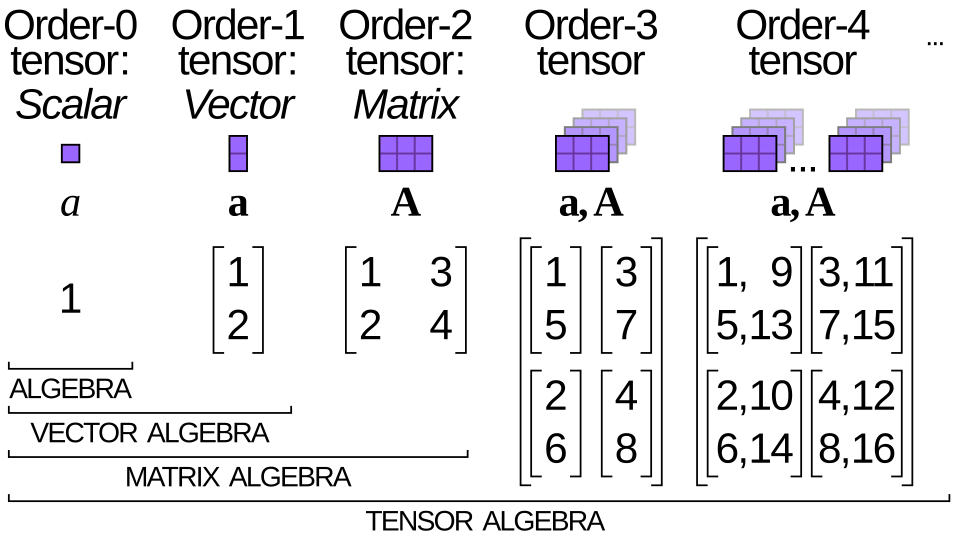
\includegraphics[width=0.8\columnwidth]{media/Tensor_dimensions.png}
    \caption{\parbox{0.8\columnwidth}{
        Illustration of tensors as a generalization of scalars, vectors, and matrices. Source: Wikipedia
    }}
    \label{fig:tensor-dimensions}
\end{figure}

In the context of neural networks, weight matrices are naturally represented as tensors. For example, a fully
connected layer with input dimension $d_{in}$ and $d_{out}$ has weight matrix $W \in R^{d_{in} \times d_{out}}$, which is a
rank-2 tensor. When considering multiple layers or batches, these weights can be reshaped into higher-order tensorr to exploit
multidimensional structure. An important concept in tensor algebra is the mode-$k$ product, denoted $\mathcal{X} \times kA$, which multiplies
a tensor $\mathcal{X}$ by a matrix $A$ along its $k$-th mode. This operation transforms the $k$-th dimension while preserving the structure of
other dimensions. The mode-$k$ product forms the foundation for tensor decomposition methods.

% Matrix Decomposition
\subsection{Matrix Decomposition}
Before discussing tensor decomposition, we briefly review matrix decomposition as a motivating example. The Singular Value
Decomposition (SVD) factorizes a matrix $M \in R^{m \times n}$ as:

\[
    M = U{\Sigma}V^T
\]
where $U \in \mathbb{R}^{m \times m}$ and $V \in \mathbb{R}^{n \times n}$ are orthogonal matrices, and $\Sigma \in \mathbb{R}^{m \times n}$
is a diagonal matrix containing singular values ${\sigma}_1 \geq {\sigma}_2 \geq \ldots \geq 0$. A low rank approximation can
be obtained by truncating the SVD to keep only the $r$ largest singular values:

\[
    M \approx M_r = U_r{\Sigma}_r{V_r}^T
\]
where $U_r \in \mathbb{R}^{m \times r}$, ${\Sigma}_r \in \mathbb{R}^{r \times r}$, and $V_r \in \mathbb{R}^{n \times r}$. This 
approximation minimizes the Frobenius norm error $||{M - M_r}||_F$ among all rank-$r$ matrices and reduces the number of parameters
from $m \times n$ to $r(m + n + 1)$. For large matrices where $r \ll min(m, n)$, this represents substantial parameter reduction.

%Tucker Decomposition
\subsection{Tucker Decomposition}
The Tucker decomposition extends the concept of low rank matrix approximation to higher order tensors. For a third-order tensor
$\mathcal{X} \in\mathbb{R}^{n_1 \times n_2 \times n_3}$, the Tucker decomposition expresses it as:

\[
    \mathcal{X}
    =
    \mathcal{G}
    \times_1 U^{(1)}
    \times_2 U^{(2)}
    \times_3 U^{(3)}
\]
where $\mathcal{G} \in\mathbb{R}^{n_1 \times n_2 \times n_3}$ is the core tensor, and $U^{(k)} \in \mathbb{R}^{n_k \times r_k}$ are
factor matrices for each mode $k$. The core tensor contains the interactions between different modes, while the factor matrices
represent principal components along each dimension.

\begin{figure}[htbp]
    \centering
    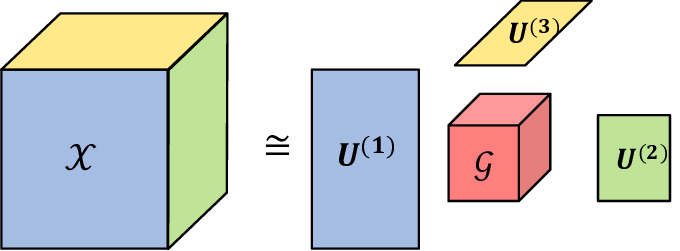
\includegraphics[width=0.8\columnwidth]{media/Tucker_decomposition_2.png}
    \caption{\parbox{0.8\columnwidth}{
        Tucker decomposition of a third order tensor into a smaller core tensor and three factor matrices along each mode. Source: ResearchGate \cite{researchgate:tucker}.
    }}
    \label{fig:tucker-decomposition}
\end{figure}

The dimensions ($r_1, r_2. r_3$) are called the multilinear rank of the tensor and control the compression level. When
$r_k \ll n_k$ for all models. Tucker decomposition achieves significant parameter reduction. For instance, the original tensor
contains $n_1 n_2 n_3$ parameters, while the Tucker representation requires only $r_1 r_2 r_3 + \sum_{k=1}^{3} n_k r_k$ parameters.

Tucker decomposition can be computed using the Higher-Order SVD (HOSVD) algorithm, which applies SVD to each mode-$k$ unfolding
of the tensor sequentially. This method guarantees orthogonal factor matrices and provides a straightforward way to truncate each
mode independently.

%Tensor-Train Decomposition
\subsection{Tensor-Train Decomposition}
The Tensor-Train (TT) decomposition offers an alternative factorization that is particularly efficient for high order tensors.
For a $d$-dimensional tensor $\mathcal{A} \in \mathbb{R}^{n_1 \times n_2 \times \ldots n_d}$, the TT decomposition represents it as:

\[
    \mathcal{A}(i_1, i_2, \ldots, i_d) = G_1(i_1) G_2(i_2) \ldots G_d(i_d)
\]
where each $G_k(i_k) \in \mathbb{R}^{r_{k-1} \times r_k}$ is a matrix slice from a third order tensor (called as TT-core), with
boundary conditions $r_0 = r_d = 1$. The values ($r_1, r_2, \ldots, r_{d-1}$) are called TT-ranks and determine the compression level.

The TT decomposition can be computed efficiently using TT-SVD algorithm, which performs $d$ sequential SVDs on reshaped versions
of the tensor. The total number of parameters in a TT representation is $\sum_{k=1}^{d} n_k r_{k-1} r_k$, which grows linearly
with the tensor order $d$ when TT-ranks are bounded. This makes TT decomposition particularly suitable for very high dimensionla
problems where Tucker decomposition would be prohibitive. One advantage of TT decomposition over Tucker is that it avoids the core
tensor, which can become a bottleneck when the tensor order is large. Additionally, TT decomposition provides a unique sequential
structure that aligns well with chain structured computations in neural networks.


% ________________________________________________________________________________________________________________

\section{Transformer Architecture and Compression Targets}

% Overview of Transformer Models
\subsection{Overview of Transformer Models}
The transformer architecture, introduced by Vaswani et al. in "Attention is All You Need," has become the foundation for modern
natural language processing models. Unlike recurrent neural networks, transformers process entire sequences in parallel using
self attention mechanisms and allowing them to capture long range dependencies efficiently.  A typical transformer model consists
of stacked blocks, each containing two primary components, a multi-head self-attention (MHA) layer and a feed-forward network (FFN).
Each block also includes residual connections and layer normalization to stabilize training. The input to a transformer begins as
token embeddings, which are augmented with positional encodings to preserve sequence order information.

\begin{figure}[htbp]
    \centering
    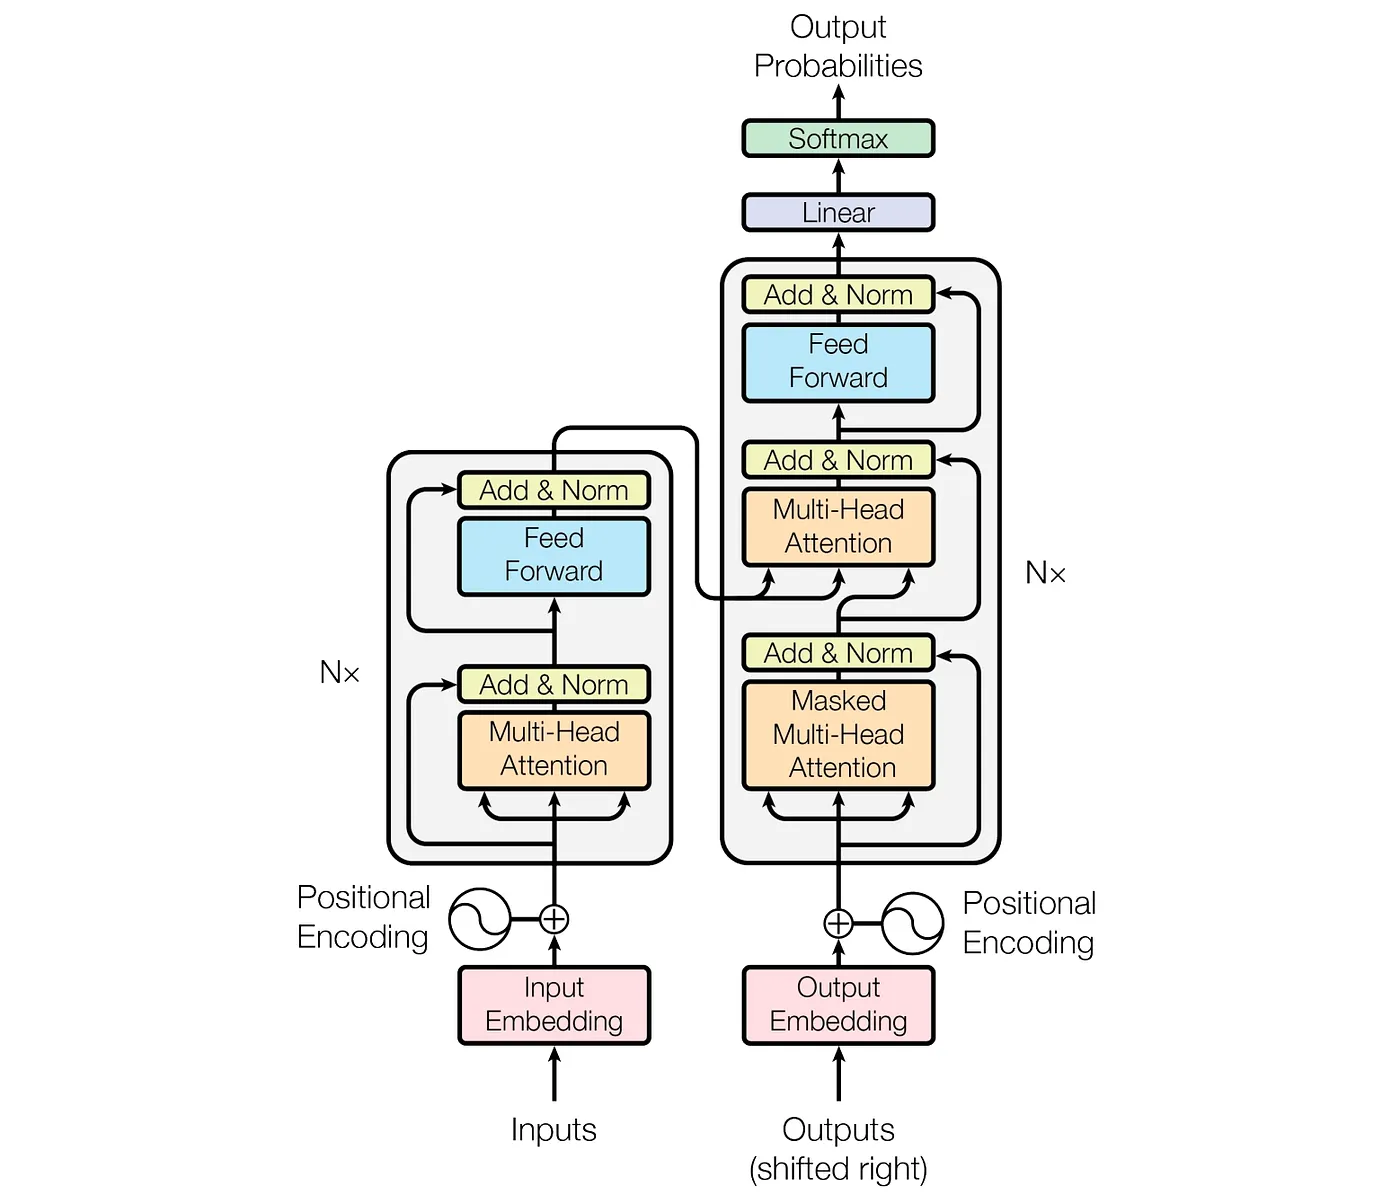
\includegraphics[width=\columnwidth]{media/Transformer_overview.png}
    \caption{\parbox{0.8\columnwidth}{
        Schematic diagram of a standard transformer block with multi-head self-attention (MHA), feed-forward network (FFN). Source: Medium \cite{medium:transformer}.
    }}
    \label{fig:transformer-overview}
\end{figure}

% Multi-Head Self-Attention Mechanism
\subsection{Multi-Head Self-Attention Mechanism}
The self-attention mechanism allows each token in a sequence to attend to all other tokens, computing relevance scores that determine
how much each token should influence the representation of others. For an input sequence represented as a matrix
$X \in \mathbb{R}^{n \times d_{model}}$, where $n$ is the sequence length and $d_{model}$ is the embedding dimension, the attention 
operation computes three matrices, quearies ($Q$), keys ($K$), and values ($V$).

These matrices are obtained through learned linear projections:

\[
    Q = XW^Q, \quad K = XW^K, \quad V = XW^V
\]
where $W^Q, W^K, W^V \in \mathbb{R}^{d_{model} \times d_k}$ are learned weight matrices. The attention scores are computes as

\[
    Attention(Q, K, V) = softmax(\dfrac{QK^T}{\sqrt{d_k}})V
\]

The scaling factor $\sqrt{d_k}$ prevents the dot products from becoming too large, which could lead to vanishing gradients during
training. Multi head attention extends this mechanism by running $h$ parallel attention operations, each with different learned projection
matrices. The outputs from all heads are concatenated and projected through another learned matrix
$W^O \in \mathbb{R}^{hd_v \times d_{model}}$ to produce the final output. For a model with $h$ attention heads, the total number
of parameters in the MHA layer is $4 \times {d_{model}}^2$ (considering $Q, K, V$, and output projections).

% Feed-Forward Networks
\subsection{Feed-Forward Networks}
Following the attention layer, each transformer block contains a positive wise feed-forward network that applies the same transformation
independently to each token position. The standard FFN consists of two linear transformations with a non-linear activation function
(typically ReLU or GELU) in between:

\[
FFN(x) = max(0, xW_1 + b_1)W_2 + b_2
\]
where $W_1 \in \mathbb{R}^{d_{model} \times d_{ff}}$ and $W_2 \in \mathbb{R}^{d_{ff} \times d_{model}}$, with $d_{ff}$ typically set
to $4d_{model}$. This means the FFN first projects the input to a higher dimensional space and then projects it back to the original
dimension.

The FFN layer contains significantly more parameters than the attention layer. Specifically, it has
$2 \times d_{model} \times d_{ff} = 8 \times {d_{model}}^2$ parameters (when $d_{ff} = 4d_{model}$), which is twice the parameter
count of the MHA layer. Research has shown that FFN layers play a crucial role in preventing representation degeneration and enabling
the model to learn complex patterns.

% Parameter Distribution and Compression Targets
\subsection{Parameter Distribution and Compression Targets}
In a standard transformer block, the parameter distribution is heavily skewed toward the FFN layers. For a model with $d_{model} = 512$,
a single transformer block contains approximately:
\begin{itemize}
    \item MHA layer: $4 \times 512^2 \approx 1.05$ million parameters
    \item FFN layer: $8 \times 512^2 \approx 2.10$ million parameters
\end{itemize}
This 2:1 ratio between FFN and MHA parameters holds across different model sizes. For models like BERT-base (110M parameters) or
GPT-2 medium (345M parameters), the majority of parameters reside in the FFN layers, making them prime candidates for compression. 
The weight matrices in both MHA and FFN layers can be reshaped into higher order tensors to enable tensor decomposition.
For instance, a weight matrix $X \in \mathbb{R}^{d_{in} \times {d_{out}}}$ can be reshaped into a third order tensor
$\mathcal{W} \in \mathbb{R}^{r_1 \times r_2 \times r_3}$ where $r_1 \times r_2 \times r_3 = d_{in} \times d_{out}$. This reshaping
allows us to apply Tucker or Tensor-Train decomposition to exploit low rank structure that may not be apparent in the original matrix
form.

Given the parameter distribution, our compression strategy focuses primarily on FFN layers, which offer the greatest potential for
parameter reduction. However, we also investigate applying tensor decomposition to the projection matrices in the attention mechanism,
particularly the value and output matrices, as these contribute substantially to the overall parameter count.

% ________________________________________________________________________________________________________________

\section{Methodology}

% Tensor Decomposition Formulation for Transformer Layers
\subsection{Tensor Decomposition Formulation for Transformer Layers}
To apply tensor decomposition to transformer weights, we first reshape weight matrices into higher order tensors. For a weight matrix
$W \in \mathbb{R}^{d_{in} \times d_{out}}$, we reshape it into a third order tensor $\mathcal{W} \in \mathbb{R}^{n_1 \times n_2 \times n_3}$
where $n_1 \times n_2 \times n_3 = d_{in} \times d_{out}$. The choice of reshape dimensions depends on the target layer. For instance,
in FFN layers where $d_{in} = d_{model}$ and $d_{out} = 4d_{model}$, a natural factorization is $n_1 = d_{model}$, $n_2 = 4$, $n_3 = d_{model}$
Once reshaped, we apply either Tucker or Tensor-Train Decomposition. For Tucker decomposition, we compute:

\[
    \mathcal{X}
    \approx
    \mathcal{G}
    \times_1 U^{(1)}
    \times_2 U^{(2)}
    \times_3 U^{(3)}
\]
where $\mathcal{G} \in \mathbb{R}^{r_1 \times r_2 \times r_3}$ is the core tensor and $U^{(k)}$ are factor matrices with rank $r_k$.
For Tensor-Train Decomposition, we apply the TT-SVD algorithm to obtain cores $G_1, G_2, G_3$ with TT-ranks $r_1, r_2$:

\[
W' = reshape(\mathcal{W}, d_{in} \times d_{out})
\]
and used directly in the forward pass without materializing the full tensor.

\begin{algorithm}[htbp]
\caption{Tensor Decomposition of a Single Transformer Layer}
\label{alg:tensor-decomposition}
\begin{algorithmic}[1]
\STATE \textbf{Input:} Weight matrix $W \in \mathbb{R}^{d_{\text{in}} \times d_{\text{out}}}$,
target tensor shape $(n_1, n_2, n_3)$ with $n_1 n_2 n_3 = d_{\text{in}} d_{\text{out}}$,
target rank parameters (e.g., $r$ or $(r_1, r_2, r_3)$),
decomposition type (Tucker or TT)
\STATE \textbf{Output:} Decomposed representation of $W$ and approximated weight matrix $W'$
\STATE
\STATE Reshape $W$ into tensor $\mathcal{W} \in \mathbb{R}^{n_1 \times n_2 \times n_3}$
\IF{decomposition type is \textit{Tucker}}
    \STATE Choose multilinear ranks $(r_1, r_2, r_3)$ based on the target compression level
    \STATE Compute Tucker decomposition
    \STATE \quad $\mathcal{W} \approx \mathcal{G} \times_1 U^{(1)} \times_2 U^{(2)} \times_3 U^{(3)}$
    \STATE \quad where $\mathcal{G} \in \mathbb{R}^{r_1 \times r_2 \times r_3}$ and
    $U^{(k)} \in \mathbb{R}^{n_k \times r_k}$ for $k = 1,2,3$
    \STATE Store core tensor $\mathcal{G}$ and factor matrices $U^{(1)}, U^{(2)}, U^{(3)}$
\ELSIF{decomposition type is \textit{Tensor-Train (TT)}}
    \STATE Choose TT-ranks $(r_1, r_2)$ (or generally $(r_1, \ldots, r_{d-1})$ for order-$d$ tensors)
    \STATE Apply TT-SVD to obtain TT-cores $G_1, G_2, G_3$ such that
    \STATE \quad $\mathcal{W}(i_1, i_2, i_3) \approx G_1(i_1) G_2(i_2) G_3(i_3)$
    \STATE Store TT-cores $G_1, G_2, G_3$
\ENDIF
\STATE Reconstruct approximated tensor $\mathcal{W}'$ from the stored factors or TT-cores
\STATE Reshape $\mathcal{W}'$ back to matrix form $W' \in \mathbb{R}^{d_{\text{in}} \times d_{\text{out}}}$
\RETURN Decomposed factors/cores and approximated matrix $W'$
\end{algorithmic}
\end{algorithm}

% Selective Layer-Wise Rank Selection
\subsection{Selective Layer-Wise Rank Selection}
Rather than applying uniform compression across all layers, we employ a selective layer wise rank selection strategy that determines
appropiate ranks per layer based on sensitivity analysis. The motivation is that different layers contribute differently to model
performance, some layers are more tolerant to low rank approx than others. Our selection procedure follows these steps:

\begin{enumerate}
    \item Layer Sensitivity Analysis:
    For each layer $l$ in the transformer, we compute a sensitivity score $S_l$ that measures how much the layer's output changes
    when decomposed to a given rank. We approximate this by:
    \[
    S_l = ||W_l - W_l'||_F/||W_l||_F
    \]
    where $W_l'$ is the reconstructed weight matrix at rank $r_l$. Layers with lower sensitivity scores are better candidates
    for higher compression.

    \item Rank Search:
    For each layer, we conduct a rank search over a predefined range $r \in [r_{min}, r_{max}]$ and measure the impact on task
    accuracy using validation data. We select the rank that achieves the best balance between compression and accuracy preservation.
    This greedy approach, while not globally optimal, is computationally tractable and has been shown to work well in practice.

    \item Fine-Tuning:
    After decomposing targeted layers, we fine tune the decomposed model on the training data to recover any accuracy loss.
    Fine tuning allows the remaining parameters to adapt to the lower rank approx and often improves final accuracy beyond 
    post decomposition accuracy. The fine tuning step is crucial because it leverages the flexibility of the uncompressed layers
    to compensate for the expressiveness lost in decomposed layers.
\end{enumerate}

As summarized in Algorithm 2, our approach iteratively evaluates each target layer by testing different rank values, computing reconstruction error and validation accuracy, then selecting the rank that optimizes the trade-off between compression ratio and model performance.

\begin{algorithm}[htbp]
\caption{Selective Tensor Rank Reduction for Transformer Layers}
\label{alg:rank-selection}
\begin{algorithmic}[1]
\STATE \textbf{Input:} Pre-trained transformer model $M$, set of target layers $\mathcal{L}$, rank search range $[r_{\min}, r_{\max}]$, validation dataset $D_{\text{val}}$
\STATE \textbf{Output:} Compressed transformer model $M'$
\STATE 
\STATE Initialize $M' \leftarrow M$
\FOR{each layer $\ell \in \mathcal{L}$}
    \STATE Obtain weight matrix $W_\ell$ from layer $\ell$
    \STATE Reshape $W_\ell$ into tensor $\mathcal{W}$ with suitable dimensions
    \STATE Initialize best rank $r_\ell^* \leftarrow r_{\max}$, best score $s_\ell^* \leftarrow -\infty$
    \FOR{$r$ from $r_{\min}$ to $r_{\max}$}
        \STATE Apply tensor decomposition (Tucker or TT) to $\mathcal{W}$ with rank $r$, obtain factors $\{\mathcal{G}, U^{(k)}\}$ or TT-cores $\{G_k\}$
        \STATE Reconstruct approximated weight $\tilde{W}_{\ell,r}$ from the decomposed factors
        \STATE Compute relative reconstruction error
        \STATE \quad $E_{\ell,r} = \|\mathcal{W} - \tilde{W}_{\ell,r}\|_F / \|\mathcal{W}\|_F$
        \STATE Temporarily replace $W_\ell$ in $M'$ with $\tilde{W}_{\ell,r}$
        \STATE Evaluate validation accuracy $A_{\ell,r}$ of $M'$ on $D_{\text{val}}$
        \STATE Compute score
        \STATE \quad $s_{\ell,r} = A_{\ell,r} - \lambda E_{\ell,r}$ \quad // $\lambda$ balances accuracy vs. compression
        \IF{$s_{\ell,r} > s_\ell^*$}
            \STATE Update $s_\ell^* \leftarrow s_{\ell,r}$, $r_\ell^* \leftarrow r$, and store $\tilde{W}_{\ell,r}$
        \ENDIF
    \ENDFOR
    \STATE Set final decomposed weight for layer $\ell$: $W_\ell \leftarrow \tilde{W}_{\ell,r_\ell^*}$ in $M'$
\ENDFOR
\STATE Fine-tune compressed model $M'$ on training data
\RETURN $M'$
\end{algorithmic}
\end{algorithm}


% Implementation Details
\subsection{Implementation Details}
We implement tensor decomposition using the Tensorly library, a Python package for tensor operations. For Tucker decomposition,
we use the Higher-Order SVD (HOSVD) algorithm, which sequentially applies SVD to mode-$k$ unfoldings. For Tensor-Train decomposition,
we use the TT-SVD algorithm with a user specified error bound $\epsilon$ which automatically determines ranks to satisfy the
approximation error constraint. The decomposition is applied selectively to
\begin{enumerate}
    \item FFN layers: All weight matrices ($W_1$ and $W_2$)
    \item Attention layers: The value and output projection matrices ($W^V$ and $W^O$) which have the highest parameter counts
\end{enumerate}
We exclude the query and key projection matrices from decomposition as preliminary experiments showed they are more sensitive to
rank reduction.


% Evaluation Metrics
\subsection{Evaluation Metrics}
We measure compression effectiveness using three key metrics:
\begin{itemize}
    \item Parameter Reduction Ratio (PRR):
        \[
        \mathrm{PRR}
        = \frac{P_{\text{orig}} - P_{\text{comp}}}{P_{\text{orig}}} \times 100\%
        \]
        where $P$ is parameters.
    \item Inference Latency Speedup:
        \[
        \mathrm{Speedup}
        = \frac{\text{Original inference time}}
            {\text{Compressed inference time}}
        \]
        Measured on a single GPU with batch size 32 over 100 test samples.
    \item Classification Accuracy:
    We report the accuracy of the compressed model on the test set of the downstream task (sentiment analysis), compared to the
    original baseline. The ultimate goal is maximize PRR and Speedup while maintaining accuracy within acceptable threshold
    (typically $< 2\%$ loss).
\end{itemize}

% ________________________________________________________________________________________________________________

\section{Experiments and Results}

% Experimental Setup
\subsection{Experimental Setup}
To evaluate the proposed compression method, we conduct experiments on the Stanford Sentiment Treebank 2 (SST-2) dataset,
a widely used benchmark for binary sentiment classification. SST-2 consists of short sentences labeled as either positive
or negative, with predefined training, validation, and test splits. Basic preprocessing is handled by the tokenizer
associated with the chosen transformer model, including lowercasing, subword tokenization, and truncation to a fixed maximum
sequence length.

As the base model, we use a pre-trained DistilBERT variant fine tuned for sentiment analysis, which provides a compact
representative transformer architecture with six layers and a hidden size of 768. This choice allows us to study
tensor based compression on a realistic transformer while keeping training and inference costs manageable.
All experiments are implemented in PyTorch using the HuggingFace Transformers library for model loading and training,
and TensorLy for tensor decomposition operations. Unless otherwise stated, models are trained and evaluated on a single
GPU with mini-batch training and early stopping based on validation accuracy.

% Baseline and Compression Settings
\subsection{Baseline and Compression Settings}
We compare three model variants in our experiments. The Baseline model is the original DistilBERT sentiment classifier
without any compression applied. The TD-FFN model applies tensor decomposition only to the feed-forward network (FFN)
layers in each transformer block, targeting the two large linear transformations that dominate the parameter count.
The TD-FFN+ATTN model extends this approach by compressing the value projection matrix $W^V$ and the output matrix $W^O$
in the multi head attention mechanism, while leaving the more sensitive query and key projections unchanged,
as motivated in Section III and IV.

For each target linear layer, we reshape the weight matrix into a third order tensor and apply Tucker or Tensor-Train
decomposition following the procedure in Algorithm 1. The candidate tensor ranks for each layer are selected from a small
discrete set (e.g. $\{16, 32, 64, 128\}$), and the final rank per layer is chosen using the selective layer wise rank
selection strategy described in Algorithm 2. This strategy balances reconstruction error and validation accuracy,
ensuring that layers with higher sensitivity receive higher ranks, while less critical layers are compressed
more aggressively. All compressed models are fine-tuned for a few epochs after decomposition to recover potential
performance loss.

% Experimental Procedure
\subsection{Experimental Procedure}
The overall experimental workflow for all model variants is summarized in Algorithm 3.

\begin{algorithm}[htbp]
\caption{End-to-End Experimental Procedure}
\label{alg:training-evaluation}
\begin{algorithmic}[1]
\STATE \textbf{Input:} Dataset $\mathcal{D}$, pre-trained model $\mathcal{M}$, compression settings (FFN/ATTN, rank $r$)
\STATE \textbf{Output:} Performance metrics for all model variants
\STATE
\STATE Split $\mathcal{D}$ into $\mathcal{D}_{\text{train}}, \mathcal{D}_{\text{val}}, \mathcal{D}_{\text{test}}$
\STATE
\STATE Train baseline: Fine-tune $\mathcal{M}$ on $\mathcal{D}_{\text{train}}$, evaluate on $\mathcal{D}_{\text{test}}$
\STATE
\FOR{each variant $v \in \{\text{TD-FFN}, \text{TD-FFN+ATTN}\}$}
    \STATE Create $\mathcal{M}_v$ by applying Algorithms 1--2 to selected layers of $\mathcal{M}$ with rank $r$
    \STATE Fine-tune $\mathcal{M}_v$ on $\mathcal{D}_{\text{train}}$ for reduced epochs
    \STATE Measure parameters, latency, and test accuracy of $\mathcal{M}_v$
\ENDFOR
\STATE
\RETURN metrics for baseline and all variants
\end{algorithmic}
\end{algorithm}

The overall experimental workflow, which integrates the compression procedures from Algorithms 1 and 2 with model training and evaluation, is summarized in Algorithm 3.

% Results
\subsection{Results}
Table I presents the comprehensive performance comparison of the baseline DistilBERT model and the two compressed variants
on the SST-2 sentiment analysis task. The results demonstrate that selective tensor rank reduction achieves substantial
parameter reduction and inference speedup, though with a moderate trade-off in classification accuracy.

\begin{table}[htbp]
\caption{Performance Comparison on SST-2}
\begin{center}
\begin{tabular}{|l|r|r|r|r|r|}
\hline
\textbf{Model} & \textbf{Params} & \textbf{PRR} & \textbf{Latency} & \textbf{Speed} & \textbf{Acc} \\
 & \textbf{(M)} & \textbf{(\%)} & \textbf{(ms)} & \textbf{up} & \textbf{(\%)} \\
\hline
Baseline & 66.96 & 0.0 & 81.22 & 1.00 & 88.65 \\
\hline
TD-FFN & 41.59 & 37.9 & 39.20 & 2.07 & 80.28 \\
\hline
TD-FFN & 35.69 & 46.7 & 30.62 & 2.65 & 77.41 \\
+ATTN & & & & & \\
\hline
\end{tabular}
\label{tab:results}
\end{center}
\end{table}

\begin{figure}[htbp]
    \centering
    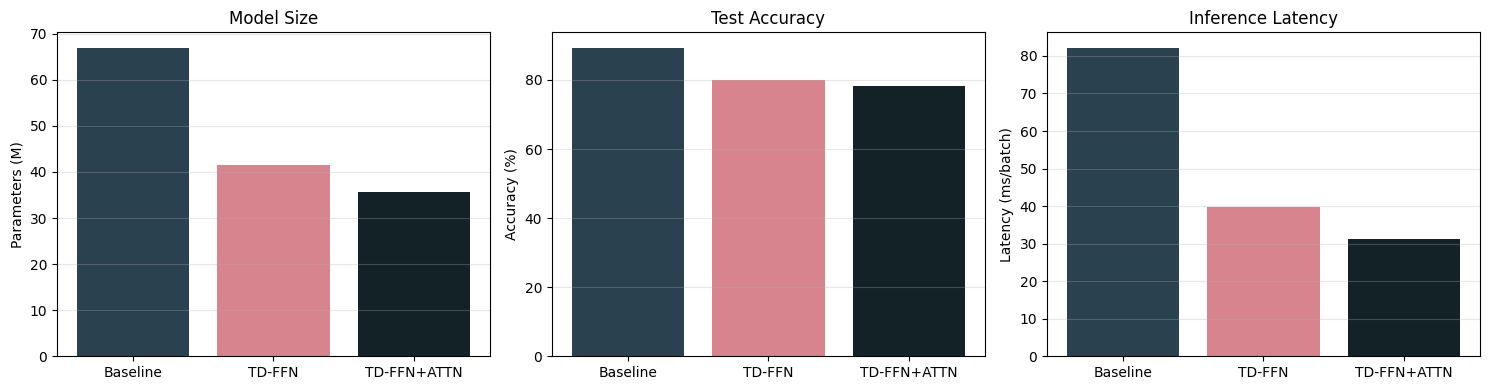
\includegraphics[width=\columnwidth]{media/output_res.png}
    \caption{\parbox{0.8\columnwidth}{
        Comparative visualization of model performance across three metrics. Source: Writter
    }}
    \label{fig:results}
\end{figure}

\begin{itemize}
    \item Parameter Reduction and Model Size: \\
            The TD-FFN model, which applies low-rank factorization exclusively to feed-forward network layers, achieves a 37.9\%
            reduction in total parameters, decreasing from 66.96M to 41.59M parameters. This aligns well with our architectural
            analysis in Section III, which identified FFN layers as the dominant contributors to parameter count in transformer
            blocks. The TD-FFN+ATTN model, which additionally compresses the value and output projection matrices in attention
            layers, achieves an even higher reduction of 46.7\%, bringing the total parameter count down to 35.69M.
            These results confirm that the proposed selective compression strategy effectively targets the most parameter-heavy
            components while preserving the overall model structure.
    \item Inference Latency and speedup:\\
            Both compressed models demonstrate significant improvements in inference speed. The TD-FFN model achieves a 2.07×
            speedup, reducing average latency from 81.22 ms/batch to 39.20 ms/batch, while the TD-FFN+ATTN model reaches 2.65×
            speedup with 30.62 ms/batch. These speedups are particularly noteworthy because they exceed the parameter reduction
            ratios, suggesting that the factorized layers not only reduce memory footprint but also benefit from more efficient
            matrix operations during forward passes. This makes the compressed models especially suitable for deployment
            scenarios where inference latency is a critical constraint, such as real-time chatbot applications or edge devices
            with limited computational resources.
    \item Classification Accuracy and Trafe-offs:\\
            The baseline model achieves 88.65\% test accuracy on SST-2 after fine-tuning. The TD-FFN model maintains 80.28\%
            accuracy, representing an 8.37 percentage point drop, while the TD-FFN+ATTN model achieves 77.41\% accuracy,
            a 11.24 point drop from baseline. While these accuracy reductions are non-trivial, they remain within acceptable
            ranges for many practical applications, particularly when weighed against the substantial gains in model size and
            speed. The larger accuracy drop in TD-FFN+ATTN compared to TD-FFN suggests that attention layers, particularly the
            value and output projections, are more sensitive to rank reduction than feed-forward layers, which aligns with
            findings from prior work on transformer compression.
    \item Layer Wise Sensitivity Analysis:\\
            Our results reveal that different layer types respond differently to low rank approximation. Feed-forward networks,
            which consist of two large linear transformations with a non-linearity in between, appear more tolerant to rank
            reduction. This is likely because the intermediate activation introduces non-linearity that can partially compensate
            for the reduced expressiveness of factorized weights. In contrast, attention mechanisms rely heavily on precise
            query-key-value interactions to capture semantic relationships, making them more sensitive to compression.
            Notably, we excluded query and key projections from compression based on preliminary sensitivity tests, which
            showed that these components are critical for maintaining attention score quality.
    \item Practical Implications:\\
            For practitioners seeking to deploy transformer-based sentiment classifiers in resource-constrained environments,
            our results suggest that the TD-FFN configuration offers the best balance between compression and accuracy.
            With a 37.9\% parameter reduction, 2.07× speedup, and only an 8.37-point accuracy drop, this variant is well suited
            for applications where moderate accuracy loss is acceptable in exchange for significant resource savings.
            The TD-FFN+ATTN model, while achieving higher compression (46.7\%) and faster inference (2.65×), may be more
            appropriate for scenarios where speed is paramount and accuracy requirements are less stringent, such as large scale
            batch processing or preliminary filtering tasks. It is worth noting that the accuracy drops observed in our
            experiments could potentially be mitigated through additional fine-tuning epochs, more sophisticated rank
            selection strategies such as layer-wise sensitivity-guided rank assignment, or hybrid approaches that combine
            tensor decomposition with other compression techniques like quantization or pruning. Future work could explore
            these directions to further optimize the compression-accuracy trade-off.

\end{itemize}

% ________________________________________________________________________________________________________________

% CONCLUSION
\section{Conclusion}
This paper presents a systematic approach to compressing transformer based language models through selective tensor decomposition
applied to feed-forward and attention layers. We formulated the compression problem as a tensor rank minimization task and
developed a layermwise rank selection algorithm that balances reconstruction accuracy with model performance. Our methodology
specifically targets the feed-forward network layers, which dominate the parameter count in transformer architectures, while
selectively compressing value and output projections in multi-head attention mechanisms.

Experimental validation on the SST-2 sentiment classification benchmark using DistilBERT demonstrates that our approach achieves
substantial resource efficiency gains. The TD-FFN variant reduces model parameters by 37.9\% and achieves a 2.07× inference
speedup with an 8.37 percentage point accuracy drop, while the more aggressive TD-FFN+ATTN configuration delivers 46.7\% parameter
reduction and 2.65× speedup at the cost of an 11.24 point accuracy decline. These results indicate that tensor decomposition offers
a practical trade-off between model size, inference speed, and predictive performance, making it particularly suitable for deployment
in resource-constrained environments such as mobile devices and edge computing platforms.

The findings reveal important insights into the compressibility of different transformer components. Feed-forward networks exhibit
greater tolerance to low-rank approximation compared to attention mechanisms, suggesting that hybrid compression strategies that
apply different rank constraints to different layer types may yield better compression-accuracy trade-offs. Additionally, the
observed superlinear speedup relative to parameter reduction indicates that factorized layers benefit from computational efficiencies
beyond simple parameter count reduction, likely due to improved memory access patterns and matrix multiplication optimization.

Future research directions include extending this framework to larger language models such as GPT and BERT-large, where the
potential for compression is significantly greater. Investigating adaptive rank selection methods that automatically determine
optimal ranks per layer based on validation performance could further improve the compression-accuracy trade-off. Additionally,
combining tensor decomposition with complementary techniques such as quantization, pruning, or knowledge distillation may enable
even higher compression ratios while maintaining model quality. Finally, exploring the application of higher-order tensor
decompositions beyond Tucker and Tensor-Train formats, such as hierarchical Tucker or tensor ring decomposition, represents a
promising avenue for future investigation.

% ________________________________________________________________________________________________________________
% \newpage


\section*{Acknowledgment}

The preferred spelling of the word ``acknowledgment'' in America is without 
an ``e'' after the ``g''. Avoid the stilted expression ``one of us (R. B. 
G.) thanks $\ldots$''. Instead, try ``R. B. G. thanks$\ldots$''. Put sponsor 
acknowledgments in the unnumbered footnote on the first page.

\section*{References}

Please number citations consecutively within brackets \cite{b1}. The 
sentence punctuation follows the bracket \cite{b2}. Refer simply to the reference 
number, as in \cite{b3}---do not use ``Ref. \cite{b3}'' or ``reference \cite{b3}'' except at 
the beginning of a sentence: ``Reference \cite{b3} was the first $\ldots$''

Number footnotes separately in superscripts. Place the actual footnote at 
the bottom of the column in which it was cited. Do not put footnotes in the 
abstract or reference list. Use letters for table footnotes.

Unless there are six authors or more give all authors' names; do not use 
``et al.''. Papers that have not been published, even if they have been 
submitted for publication, should be cited as ``unpublished'' \cite{b4}. Papers 
that have been accepted for publication should be cited as ``in press'' \cite{b5}. 
Capitalize only the first word in a paper title, except for proper nouns and 
element symbols.

For papers published in translation journals, please give the English 
citation first, followed by the original foreign-language citation \cite{b6}.

\begin{thebibliography}{00}
\bibitem{researchgate:tucker} ``Tucker decomposition of a third-order weight tensor,'' ResearchGate. [Online]. Available: https://www.researchgate.net/figure/Tucker-decomposition-of-a-third-order-weight-tensor\_fig1\_321896554. [Accessed: Dec. 24, 2025].
\bibitem{medium:transformer} ``Transformer: Attention is All You Need,'' Medium. [Online]. Available: https://dataturbo.medium.com/transformer-attention-is-all-you-need-fe6205c5be33. [Accessed: Dec. 24, 2025].
\end{thebibliography}

\end{document}
